\documentclass[tikz,border=5pt]{standalone}
\usepackage{fontspec}
\setmainfont{Times New Roman}
\usepackage{unicode-math}
\setmathfont{Cambria Math}
\usetikzlibrary{shapes.geometric,shapes.misc,positioning,fit,backgrounds,arrows.meta,calc}

\begin{document}
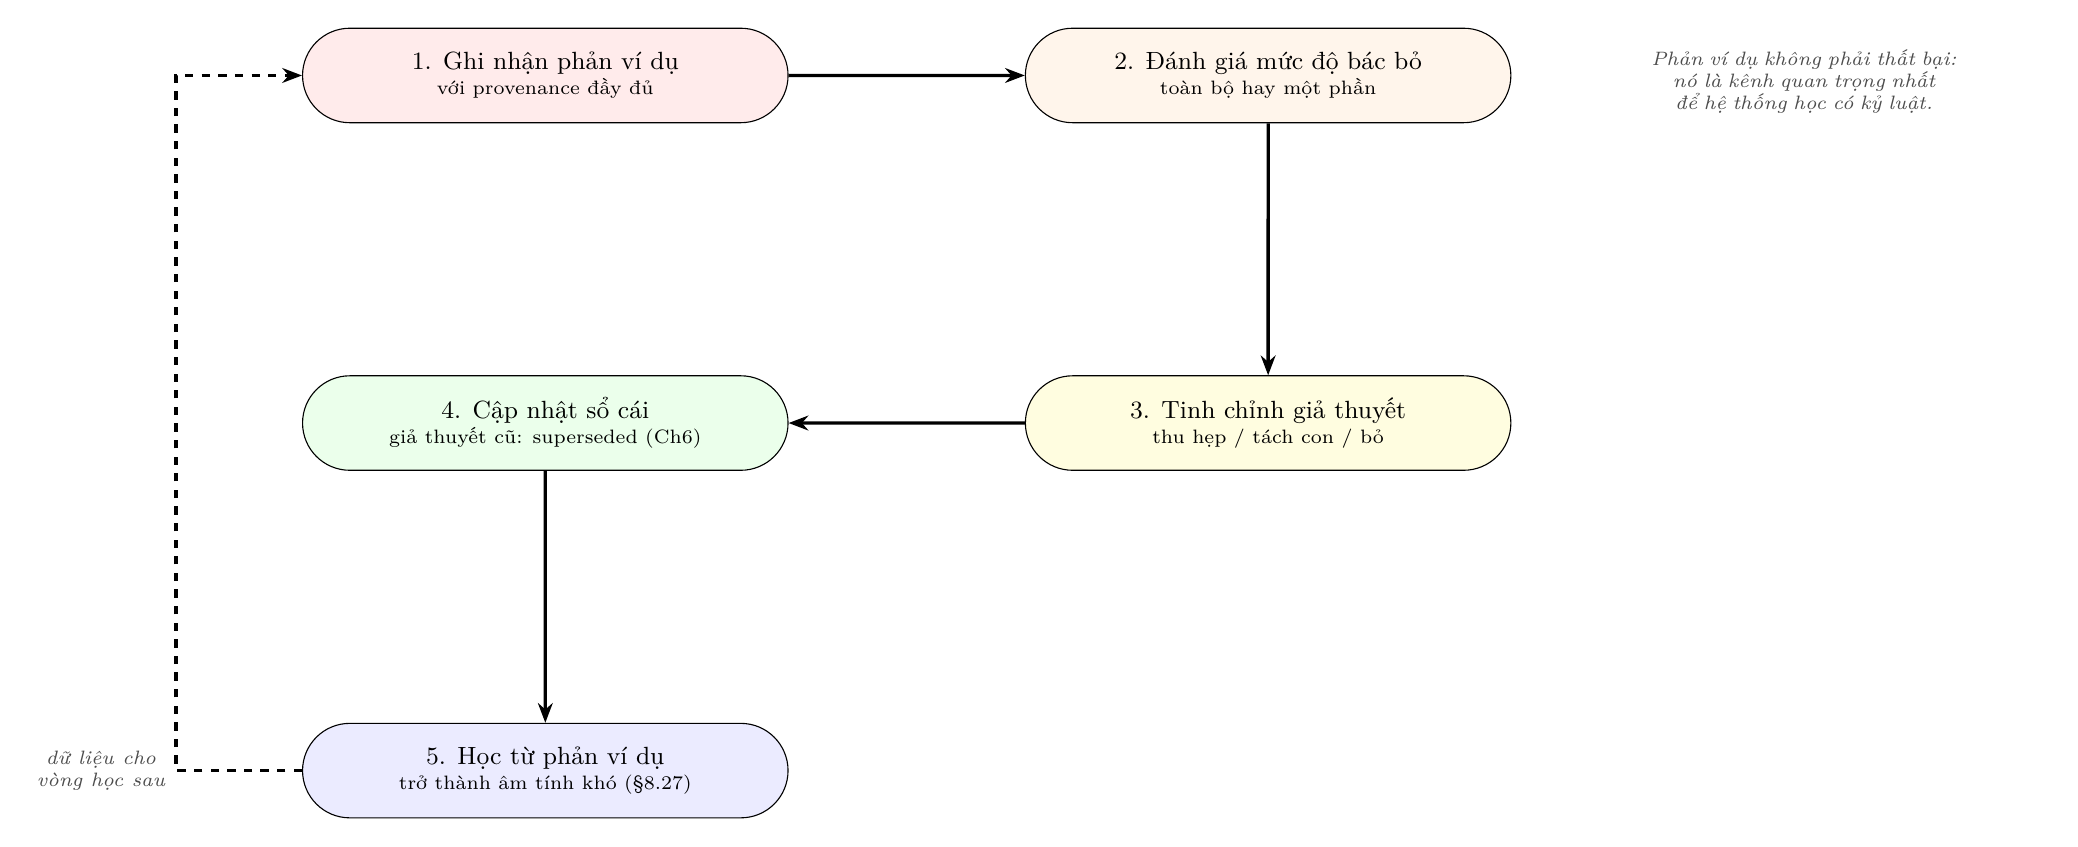
\begin{tikzpicture}[
  stage/.style={rounded rectangle, draw, align=center, minimum width=6.4cm, minimum height=1.2cm, font=\small},
  arrow/.style={-{Stealth[length=2.5mm]}, very thick},
  label/.style={font=\scriptsize\itshape, text=gray!60!black},
]

% === Counterexample loop (clockwise) ===
\node[stage, fill=red!8] (obs) at (0, 3.4) {1. Ghi nhận phản ví dụ\\[-2pt]\scriptsize với provenance đầy đủ};
\node[stage, fill=orange!8, right=3.0cm of obs] (assess) {2. Đánh giá mức độ bác bỏ\\[-2pt]\scriptsize toàn bộ hay một phần};
\node[stage, fill=yellow!12, below=3.2cm of assess] (refine) {3. Tinh chỉnh giả thuyết\\[-2pt]\scriptsize thu hẹp / tách con / bỏ};
\node[stage, fill=green!8, left=3.0cm of refine] (ledger) {4. Cập nhật sổ cái\\[-2pt]\scriptsize giả thuyết cũ: superseded (Ch6)};

\draw[arrow] (obs) -- (assess);
\draw[arrow] (assess) -- (refine);
\draw[arrow] (refine) -- (ledger);

% === Loop back to learning ===
\node[stage, fill=blue!8, below=3.2cm of ledger] (learn) {5. Học từ phản ví dụ\\[-2pt]\scriptsize trở thành âm tính khó (§8.27)};
\draw[arrow] (ledger) -- (learn);
\draw[arrow, dashed] (learn.west) -- ++(-1.6,0) node[label, left, align=center] {dữ liệu cho\\vòng học sau} |- (obs.west);

% === Annotation ===
\node[label, align=center, text width=6.0cm, right=1.2cm of assess.south east, anchor=south west]
  {Phản ví dụ không phải thất bại:\\ nó là kênh quan trọng nhất\\ để hệ thống học có kỷ luật.};

\end{tikzpicture}
\end{document}